\documentclass{article} % For LaTeX2e
\usepackage{nips15submit_e,times}
\usepackage{hyperref}
\usepackage{url}
\usepackage{graphicx}
\usepackage{amsfonts}
\usepackage{amssymb}
\usepackage{float}
\usepackage{listings}
\usepackage{xcolor}
\usepackage{amsmath}
%\documentstyle[nips14submit_09,times,art10]{article} % For LaTeX 2.09


\title{Problem Set 2 for Machine Learning 15 Fall}


\author{
Jingyuan Liu\\
AndrewId: jingyual\\
\texttt{jingyual@andrew.cmu.edu} \\
}


\newcommand{\fix}{\marginpar{FIX}}
\newcommand{\new}{\marginpar{NEW}}
\newcommand{\argmin}{\arg\!\min}
\newcommand{\norm}[1]{\left\lVert #1 \right\rVert}
\newcommand{\abs}[1]{\left\lvert #1 \right\rvert}
\newcommand{\inner}[1]{\left\langle #1 \right\rangle}


\nipsfinalcopy % Uncomment for camera-ready version


\begin{document}
\maketitle



\section{Bayes Optimal Classification}


\subsection{Determine the Bayes optimal classifier}
Our goal is to minimize the risk, so classifier should choose the
condition that have smaller risk:

\[ f(x) =
    \begin{cases}
        1 & \qquad if \quad \alpha p(f(x)=1,y=0) < \beta p(f(x)=0,y=1) \\
        0 & \qquad if \quad \alpha p(f(x)=1,y=0) > \beta p(f(x)=0,y=1) \\
    \end{cases}
\]


\subsection{Show the $\alpha$ and $\beta$}
Using bayes rule, we can derive:

\begin{equation}
R = p(f(x) = 1 \mid y = 0) + p(f(x) = 0 \mid y = 1)
\end{equation}

\begin{equation}
\quad = \frac{p(f(x)=1, y=0)}{p(y=0)} + \frac{p(f(x)=0, y=1)}{p(y=1)}
\end{equation}

Therefore, we can choose:

\begin{equation}
\alpha = \frac{1}{p(y=0)}, \beta = \frac{1}{p(y=1)}
\end{equation}


\subsection{Classification Problem}
From the question, we would know:

\[ p(x) =
    \begin{cases}
        1-p & \qquad if \quad y = 1 \quad and \quad x = 0\\
        p   & \qquad if \quad y = 1 \quad and \quad x = 1 \\
        1-q & \qquad if \quad y = 0 \quad and \quad x = 0 \\
        q   & \qquad if \quad y = 0 \quad and \quad x = 1 \\
    \end{cases}
\]

\begin{equation}
p(y=0) = p(y=1) = \frac{1}{2}
\end{equation}

When x = 0, we should choose y = 0, because 1 - p $<$ 1 - q. When x = 1, y =1:

\begin{equation}
f(x) = x , \qquad R = p(f(x)=1, y=0) + p(f(x)=0, y=1) = \frac{1}{2} (1-p+q)
\end{equation}



\section{Regularized Linear Regression Using Lasso}


\subsection{Show the J(w)}
The goal is to find the w that minimize the error:
\begin{equation}
w^{\star} = \argmin_w \frac{1}{2} \norm{ y - Xw }^2 + \lambda \norm{ w }_1
\end{equation}

Therefore, to write in the form as required:

\begin{equation}
J_{\lambda} (w) = \frac{1}{2} \norm{ y - Xw }^2 + \lambda \norm{ w }_1
\end{equation}

\begin{equation}
= \frac{1}{2} \sum_k^n (y_k - \sum_i^d w_i X_{ki})^2 + \lambda \sum_i \abs{w_i}
\end{equation}

\begin{equation}
\qquad \qquad \qquad \qquad = \frac{1}{2} \sum_k^n (y_k^2 - 2 y_k \sum_i^d w_i X_{ki}
+ (\sum_i^d w_i X_{ki})^2) + \lambda \sum_i^d \abs{w_i}
\end{equation}

As it notices that $X^T X = I$, so:

\begin{equation}
J_{\lambda} (W)= \frac{1}{2} \sum_k^n (y_k^2 - 2 \sum_i^d y_k w_i X_{ki} + \sum_i^d w_i^2)
+ \lambda \sum_i^d \abs{w_i}
\end{equation}

So to transfer to the form, we have:

\begin{equation}
g(y) = \frac{1}{2} y^2 , \qquad f(X_{.i}, y, w_i, \lambda) =
\frac{1}{2} ((w_i^2  - 2 y X_{.i} w_i) + \lambda \abs{w_i}
\end{equation}


\subsection{Find $w_i^{\star}$ when $w_i^{\star} > $ 0}
As the previous function shows, and $w_i >$ 0, we can have:

\begin{equation}
\frac{\partial J(W)}{\partial w_i} = w_i - (yX_i - \lambda) 
\end{equation}

The $w_i^{\star}$ is the best $w_i$ that would make the J (w) smallest:

\[ w_i^{\star} =
    \begin{cases}
        yX_i - \lambda & \qquad if \quad yX_i > \lambda \\
        0              & \qquad if \quad yX_i < \lambda \\
    \end{cases}
\]

If $yX_i < \lambda$, then the minimal point that the gradient is zero could not
be reached by the qudartic curve. Under this condition, the smaller the $w_i$,
the smaller the J(w), so $w_i$ = 0.


\subsection{Find $w_i^{\star}$ when $w_i^{\star} < $ 0}
Similarily, we can get $w_i^{\star}$ under this condition:

\begin{equation}
\frac{\partial J(W)}{\partial w_i} = w_i - (yX_i + \lambda)
\end{equation}

\[ w_i^{\star} =
    \begin{cases}
        yX_i + \lambda & \qquad if \quad yX_i < -\lambda \\
        0              & \qquad if \quad yX_i > -\lambda \\
    \end{cases}
\]


\subsection{Find Condition $w_i^{\star}$ = 0}
To conlude, under the two conditions, if we want the $w_i^{\star}$ be zero, we
would need:

\[ \lambda =
    \begin{cases}
        \lambda < -yX_i   & \qquad if \quad yX_i < 0 \quad and \quad w_i <= 0 \\
        \lambda >  yX_i   & \qquad if \quad yX_i > 0 \quad and \quad w_i >= 0 \\
    \end{cases}
\]

\begin{equation}
\lambda > \abs{yX_i}
\end{equation}

We could find that this is really very reasonable answer, because adding lasso
is to get a sparse parameter vector as mentioned. We could find that given a
certain $\lambda$, if the absolute product of feature i and y $yX_i$ is smaller
than $\lambda$ would be 0 to achieve the minimal likelihood J(W). With the
lasso, those weights of features with ``small'' would temp to go to zero in the
training.


\subsection{Ridge Regression}
As mentioned, we can have:

\begin{equation}
J_{\lambda} (W)= \frac{1}{2} \sum_k^n (y_k^2 - 2 \sum_i^d y_k w_i X_{ki} + \sum_i^d w_i^2)
+ \lambda \sum_i^d \norm{w_i}^2
\end{equation}

\begin{equation}
\frac{\partial J(W)}{\partial w_i} = (1+\lambda) w_i - yX_i
\end{equation}

So if we want $w_i = 0$, then we need $yX_i = 0$. This is different from
condition 4. Because the value of $w_i = 0$ only deepends y and $X_i$.


\section{Multinomial Logistic Regression}

\subsection{Show the special form, logistic regression}
Suppose the C = 2, then we have:

\begin{equation}
p(y=c^0 \mid x, W) = \frac{exp(w_{c0}^0 + w_{c}^{0T} x)}
{exp(w_{c0}^0 + w_{c}^{0T} x) + {exp(w_{c0}^1 + w_{c}^{1T} x})}
\end{equation}

\begin{equation}
p(y=c^1 \mid x, W) = \frac{exp(w_{c0}^1 + w_{c}^{1T} x)}
{exp(w_{c0}^0 + w_{c}^{0T} x) + {exp(w_{c0}^1 + w_{c}^{1T} x})}
\end{equation}

and we could transfer to:

\begin{equation}
p(y=c^0 \mid x, W) = \frac{1}
{1 + {exp(w_{c0}^1 - w_{c0}^0+ w_{c}^{1T} x - w_{c}^{0T} x})}
\end{equation}

\begin{equation}
p(y=c^0 \mid x, W) =
\frac{exp(w_{c0}^1 - w_{c0}^0+ w_{c}^{1T} x - w_{c}^{0T} x)}
{1 + {exp(w_{c0}^1 - w_{c0}^0+ w_{c}^{1T} x - w_{c}^{0T} x})}
\end{equation}

We could see that multiclass Logistic regression reduce to logsitic
regression when C = 2.

\subsection{Multinomial Logistic Regression}
\textbf{Log Likelihood Function}

We could derive the log likelihood based on the given form:

\begin{equation}
l(W) = log (\prod_i p(y_i \mid x_i, W))
\end{equation}

\begin{equation}
\qquad \qquad \qquad = log (\prod_i \prod_c p(y_i = c \mid x_i, W))
\end{equation}

Here we could use a denotation function, $t_{ic}$:

\[ t_{ic} =
    \begin{cases}
        1 & \qquad if \quad y_i == c \\
        0 & \qquad if \quad y_i != c \\
    \end{cases}
\]

With this denotation function:

\begin{equation}
l(w) = log (\prod_i \prod_c p(y_i=c \mid x_i, W)^{t_{ic}})
\end{equation}

\begin{equation}
\qquad = \sum_i \sum_c t_{ic} log(p(y_i=c \mid x_i, W))
\end{equation}

\begin{equation}
\qquad \qquad = \sum_i \sum_c t_{ic} log ( \frac{exp(w_{c0}+w_c^T x)}{\sum_{c'}
exp(w_{c'0}+w_{c'}^T x )} )
\end{equation}

\textbf{Derive the Gradient}

To maximize the likelihood function, we need to derive the gradients for each
weight:

\begin{equation}
g_c (W) = \frac{\partial l(W)}{\partial w_c}
\end{equation}

\begin{equation}
= \frac{\partial \sum_i \sum_c t_{ic} log(p(y_i=c \mid x_i, W))}
{\partial w_c}
\end{equation}

\begin{equation}
= \sum_{i \in (y_i=c) } x_i
- \sum_i x_i \frac{exp(w_c^T x_i)}
{\sum_{c'} exp(w_{c'}^T x_i)})
\end{equation}

\textbf{Derive the Hessian}

To derive the hessian, we could do it based on the gradient:

\begin{equation}
H_{c,c'}(W) = \frac{\partial^2 l(W)}{\partial w_c \partial w_{c'}}
\end{equation}

\begin{equation}
\qquad \qquad = \frac{\partial g_c (W)}{\partial w_{c'}}
\end{equation}

\begin{equation}
\qquad \qquad \qquad \qquad \qquad \qquad \qquad = \frac{\partial \sum_i x_i (1 - p(y_i = c \mid x_i, W))}
{\partial w_{c'}}
\end{equation}

\[=
    \begin{cases}
        \sum_i x_i^2 p(y_i=c \mid x_i,W) (p(y_i=c' \mid x_i,W)-1) & \quad if \quad c == c' \\
        \sum_i x_i^2 p(y_i=c \mid x_i,W) p(y_i=c' \mid x_i,W) & \quad if \quad c != c' \\
    \end{cases}
\]



\section{Perceptron Mistake Bounds}


\subsection{Show that $\inner{w^t, w} >= t \gamma$}
\begin{equation}
\inner{w^t, w} = \inner{w_{t-1} + y^t x^t,w}
\end{equation}

\begin{equation}
= \inner{w^{t-1},w} + \inner{y^t x^t, w}
\end{equation}

\begin{equation}
>= \inner{w^{t-1},w} + \gamma
\end{equation}

We can continously derive $\inner{w^{t-1}, w}$ to $w^0$, and there will be total
t items. Therefore, we could

\begin{equation}
\inner{w^t, w} > t \gamma
\end{equation}


\subsection{Show that $\norm{w^t}_2^2 <= tM^2$}
\begin{equation}
\norm{w^t}_2^2 = \inner{w^t,w^t}
= \inner{w^{t-1}+y^tx^t, w^{t-1}+y^tx^t}
\end{equation}

\begin{equation}
= \inner{w^{t-1},w^{t-1}} + 2 \inner{w^{t-1},y^tx^t} + \inner{y^tx^t,y^tx^t}
\end{equation}

We know that $y^t, x^t$ is the misclassified cases, therefore
$\inner{w^{t-1},y^tx^t} < 0$. And y can only be 1 or -1. So we know that
$\inner{y^tx^t, y^tx^t}$ is $\norm{x}^2_2 < M^2$. So, we have:

\begin{equation}
\norm{w^t}_2^2 <= \inner{w^{t-1},w^{t-1}} + M^2
\end{equation}

We can derive $w^t$ to $w^0$, so we have total t items, so we can prove that:

\begin{equation}
\norm{w^t}_2^2 <= tM^2
\end{equation}


\subsection{Prove the upper bound}
We know that the meaning of $\inner{a,b}$ is related the $cos(\theta)$, which is the cos
value of the angle between the vector a and b. So we have:

\begin{equation}
cos(\theta) = \frac{\inner{w^t,w}}{\norm{w_t} \norm{w}}
\end{equation}

We know that $\norm{w} = 1$, and take the form experssion into it, we have

\begin{equation}
cos(\theta) = \frac{t \gamma}{\sqrt{t} M} <= 1
\end{equation}

So we have that:

\begin{equation}
t <= \frac{M^2}{\gamma^2}
\end{equation}


\subsection{True or False}
I think it is false. There should be a lot of classifiers that achieve zero
error. But only $w = w^t$ and $t=\frac{M^2}{\gamma^2}$ will the classifier have
margin $\gamma$.



\section{Logistic Regression for Image Classification}


\subsection{Exploring the data}

Run the modified code, and look at the variables stored in the memory

\textbf{size of image}

\qquad The size of image is 784 X 8 Byte.

\textbf{range of labels}

\qquad 1 to 10

\textbf{range of pixel values}

\qquad 0 to 1

\textbf{max and min l2-norm}

\qquad max: 17.1790, min: 3.5698

\textbf{sparsity}

\qquad we could find that 80.88\% nodes are 0 value, so the data is sparse.

\textbf{uniform}

\qquad The max is 6742, the min is 5421. So it is uniformed.

\subsection{Binary Logistic Regression}

\textbf{Without Regularization}

The final objective function value is -897.275,

the $\norm{w}^2$ is 19.08,

the trainning accuracy is 0.978551

the testing accuracy is 0.968246

trainning iterations is 674

\textbf{With Regularization}

The final objective function value is -1008.07,

the $\norm{w}^2$ is 9.75082,

the trainning accuracy is 0.977466

the testing accuracy is 0.969254

trainning iterations is 326

\textbf{Conclustion}

We could find that adding regularization will lead the iteration faster to
conrvege, get higher test performances, and have smaller norm of w.


\subsection{Multiclass logistic regression}
The final objective function value is -15269.5,

the $\norm{w}^2$ is 47.7107,

the trainning accuracy is 0.931033

the testing accuracy is 0.925300

trainning iterations is 662

The visualization is as follows:

\begin{figure}[h]
\begin{center}
\label{fig:nn}
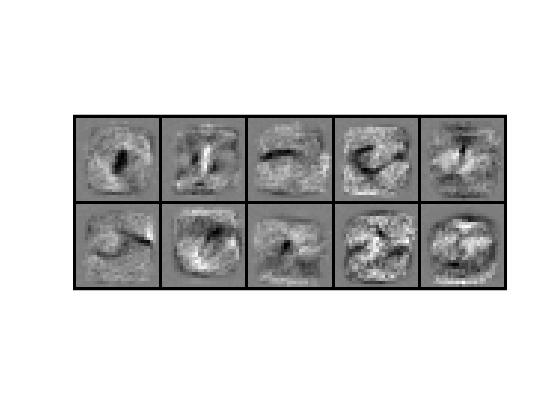
\includegraphics[width=12cm]{pic/result.jpg}
\caption{visualization}
\end{center}
\end{figure}



\section{Collaboration}
I dicussed with Zheng Chen with problem 2 on understanding finding the minimal
for a quardratic function. And discussed with him on question 4 about using the
cos value. And double checked the question 5 implementation.

\end{document}
